% Shared preamble for the Radioactive Signal Explorer explainers (docs/signals/*.tex).
\documentclass[11pt]{article}
\usepackage[letterpaper,margin=1in]{geometry}
\usepackage[T1]{fontenc}
\usepackage{lmodern}
\usepackage{microtype}
\usepackage{amsmath,amssymb,mathtools,bm}
\usepackage{siunitx}
\usepackage{graphicx}
\usepackage{booktabs,array,tabularx}
\usepackage{xcolor}
\usepackage{enumitem}
\usepackage{caption}
\usepackage[section]{placeins}
\usepackage[most]{tcolorbox}
\usepackage[colorlinks=true,linkcolor=blue!50!black,citecolor=blue!50!black,urlcolor=blue!50!black]{hyperref}
\usepackage[capitalise,noabbrev]{cleveref}
\sisetup{group-separator={,},group-minimum-digits=4,separate-uncertainty}
\definecolor{labblue}{HTML}{0088EE}
\definecolor{exbg}{HTML}{FFF7EC}
\definecolor{boxbg}{HTML}{EEF4FB}
\newtcolorbox{keyidea}[1][]{colback=boxbg,colframe=labblue,boxrule=0.6pt,arc=2pt,left=6pt,right=6pt,top=4pt,bottom=4pt,fonttitle=\bfseries,title={#1}}
\newtcolorbox{pitfall}[1][]{colback=red!3,colframe=red!55!black,boxrule=0.6pt,arc=2pt,left=6pt,right=6pt,top=4pt,bottom=4pt,fonttitle=\bfseries,title={#1}}
\newcounter{exercise}
\newtcolorbox{exercise}[1][]{colback=exbg,colframe=orange!70!black,boxrule=0.6pt,arc=2pt,left=6pt,right=6pt,top=4pt,bottom=4pt,fonttitle=\bfseries,
  title={Exercise~\refstepcounter{exercise}\theexercise\ifx\relax#1\relax\else\ (#1)\fi}}
\newcommand{\dd}{\mathrm{d}}
\newcommand{\keV}{\,\mathrm{keV}}
\newcommand{\MeV}{\,\mathrm{MeV}}
\newcommand{\me}{m_e c^2}
\newcommand{\nuc}[2]{${}^{#1}$#2}
\newcommand{\code}[1]{\texttt{#1}}
\newcommand{\explorer}{\href{https://dark-matter.ucr.edu/Signals.html}{Radioactive Signal Explorer}}
\newcommand{\seriesnote}{\noindent\small This note is one of five explaining the physics behind the \explorer: gamma rays, alpha decay, $(\alpha,n)$ neutrons, beta decay and Cherenkov light. Every figure was computed with the page's own code (\code{assets/signals-physics.js}); the \LaTeX{} sources and figure scripts are in \code{docs/signals/} of \url{https://github.com/UCRDarkMatter/dark-matter-lab-site}. Exercises are marked (A) analytic, (P) programming, (R) open-ended.\normalsize}

\title{Cherenkov Light from Radioactive Decays:\\ Frank--Tamm, Dispersion and Slowing Down}
\author{UCR Dark Matter Lab --- notes for graduate students}
\date{\today}
\begin{document}
\maketitle
\seriesnote

\begin{abstract}
Electrons from beta decays and from gamma interactions emit Cherenkov light if they move faster than light in the medium. In water, acrylic, quartz windows and PMT glass this is a source of prompt, fast light that can mimic or contaminate a scintillation signal---and in water Cherenkov detectors it is the signal. This note derives the Cherenkov condition and the Frank--Tamm spectrum, shows how to integrate it over the slowing-down of an electron and over a beta or gamma spectrum, and explains the refractive-index models and stopping powers used by the Cherenkov tab of the Signal Explorer.
\end{abstract}
\tableofcontents

\section{The Cherenkov condition}
A charged particle moving through a dielectric polarises it. If the particle moves at speed $\beta c$ greater than the phase velocity $c/n$ of light in the medium, the wavelets emitted by the polarisation along the track add coherently on a cone, exactly as a bow wave or a sonic boom. Huygens' construction gives the cone angle
\begin{equation}
\cos\theta_C = \frac{1}{n\beta},
\label{eq:angle}
\end{equation}
which has a solution only if $\beta > 1/n$. For an electron this is a kinetic-energy threshold
\begin{equation}
T_\text{th} = \me\left(\frac{1}{\sqrt{1 - 1/n^2}} - 1\right),
\label{eq:thr}
\end{equation}
\SI{257}{keV} in water ($n=1.34$), \SI{178}{keV} in acrylic ($n=1.49$), \SI{186}{keV} in fused silica ($n\approx1.47$ at \SI{400}{nm}). The maximum angle, for $\beta\to1$, is \ang{41.7} in water. Because $n$ depends on wavelength, so do the threshold and the angle; in the near UV, where $n$ rises, the threshold is lower.

\section{The Frank--Tamm formula}
Classical electrodynamics in a medium with permittivity $\epsilon(\omega) = n^2(\omega)$ gives the energy radiated per unit path length and frequency (Frank and Tamm, 1937). Dividing by $\hbar\omega$ and converting to wavelength gives the number of photons per unit path length and wavelength:
\begin{equation}
\boxed{\;\frac{\dd^2 N}{\dd x\,\dd\lambda} = \frac{2\pi\alpha z^2}{\lambda^2}\left(1 - \frac{1}{\beta^2 n^2(\lambda)}\right) = \frac{2\pi\alpha z^2}{\lambda^2}\sin^2\theta_C\;}
\label{eq:ft}
\end{equation}
for a particle of charge $ze$, and zero where $\beta n(\lambda) < 1$. Three features stand out:
\begin{itemize}
\item the $1/\lambda^2$ dependence: Cherenkov light is blue and UV, and most photons are at the shortest wavelengths the medium transmits;
\item the yield is small: for $\beta\to1$ in water, integrating from 300 to \SI{600}{nm} gives $2\pi\alpha\sin^2\theta_C(1/\lambda_1 - 1/\lambda_2) \approx \SI{330}{photons/cm}$, compared with tens of thousands of photons per MeV for a good scintillator;
\item the emission is prompt (sub-picosecond) and directional, which is what makes it useful for pulse-shape and topological discrimination.
\end{itemize}
The energy radiated is negligible compared with ionisation losses (a few keV per cm), so Cherenkov emission does not need to be included in the stopping power.

\section{Integrating over the slowing-down of an electron}
An electron of initial kinetic energy $T_0$ radiates until it falls below threshold. In the continuous-slowing-down approximation (CSDA), $\dd x = \dd T / (\rho S(T))$, where $S$ is the total mass stopping power, so the number of photons per unit wavelength is
\begin{equation}
\frac{\dd N}{\dd\lambda}(T_0) = \int_{T_\text{th}(\lambda)}^{T_0} \frac{2\pi\alpha}{\lambda^2}\left(1 - \frac{1}{\beta^2(T) n^2(\lambda)}\right)\frac{\dd T}{\rho\,S(T)} .
\label{eq:track}
\end{equation}
The explorer tabulates the cumulative integral on a fine grid of $T$ for each wavelength once (\code{cherenkovTable}), so that the yield for any starting energy is a table lookup.

\subsection{Stopping power}
For electrons the collision stopping power is given by the Bethe formula as adapted by Rohrlich and Carlson (ICRU Report 37) \cite{icru37},
\begin{equation}
S_\text{col} = \frac{2\pi r_e^2 \me N_A}{\beta^2}\,\frac{Z}{A}\left[\ln\frac{\tau^2(\tau+2)}{2(I/\me)^2} + F^-(\tau) - \delta\right],
\end{equation}
\begin{equation}
F^- = 1 - \beta^2 + \frac{\tau^2/8 - (2\tau+1)\ln2}{(\tau+1)^2},
\end{equation}
Here $\tau = T/\me$, and $I$ is the mean excitation energy, \SI{75}{eV} for water. The prefactor is \SI{0.153537}{MeV\,cm^2/g} times $(Z/A)/\beta^2$. The density-effect correction $\delta$ is negligible below a few MeV and is omitted. Radiative (bremsstrahlung) losses are added with the rule of thumb $S_\text{rad}/S_\text{col} \approx Z_\text{eff}(T + \me)$ divided by \SI{800}{MeV}; for water at \SI{2}{MeV} this is a 2\% correction. All three material constants ($\rho$, $Z/A$, $I$) are editable in the tab.

\subsection{What the CSDA leaves out}
\begin{pitfall}[Approximations in \cref{eq:track}]
\begin{itemize}[leftmargin=1em]
\item \textbf{Delta rays.} Energetic knock-on electrons above threshold also radiate. CSDA puts all losses into the primary, slightly underestimating the light for high-energy primaries.
\item \textbf{Multiple scattering} does not change the path length integral (the yield) but completely smears the cone direction for electrons of a few hundred keV: the light from a \SI{1}{MeV} electron is far from a clean ring.
\item \textbf{Range straggling}: real tracks have fluctuating lengths, so the yield fluctuates beyond Poisson statistics.
\item \textbf{Absorption and the detector}: \cref{eq:track} is the light \emph{produced}. Water absorbs strongly below \SI{200}{nm}, acrylic below about \SI{300}{nm}, and photocathode quantum efficiency and wavelength shifters decide what is detected.
\end{itemize}
\end{pitfall}

\section{Refractive index models}
The tab offers three ways to specify $n(\lambda)$:
\begin{enumerate}
\item \textbf{Constant $n$}, for quick estimates;
\item a \textbf{material preset} with a published Sellmeier fit;
\item \textbf{custom Sellmeier coefficients}.
\end{enumerate}
The Sellmeier equation models the medium as a set of oscillators with resonance wavelengths $\sqrt{C_i}$:
\begin{equation}
n^2(\lambda) = 1 + \sum_i \frac{B_i\,\lambda^2}{\lambda^2 - C_i}, \qquad \lambda \text{ in \si{\micro m}}, \ C_i \text{ in \si{\micro m^2}}.
\end{equation}
It is accurate between the UV and IR resonances and diverges as $\lambda\to\sqrt{C_i}$, so it must not be used below the fit's range (about \SI{200}{nm} for water and fused silica). The presets are water at \SI{20}{\celsius} (Daimon and Masumura \cite{daimon}), fused silica (Malitson \cite{malitson}), PMMA, BK7, sapphire (ordinary ray) and diamond. \Cref{fig:n} shows three of them. A constant $n$ underestimates the UV yield in all of them, since $n$ rises towards the UV.

\begin{figure}[htbp]
\centering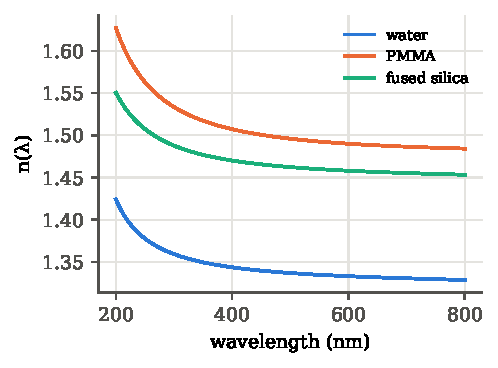
\includegraphics[width=0.6\linewidth]{fig/c_n.pdf}
\caption{Sellmeier refractive indices used by the presets. At \SI{400}{nm}, $n = 1.344$ for water.}
\label{fig:n}
\end{figure}

\section{Spectra from decays}
For a source of electrons with kinetic-energy distribution $\dd N_e/\dd T$ (per decay),
\begin{equation}
\frac{\dd N_\gamma}{\dd\lambda} = \int \frac{\dd N_e}{\dd T}(T)\;\frac{\dd N}{\dd\lambda}(T)\;\dd T .
\label{eq:fold}
\end{equation}
The tab takes $\dd N_e/\dd T$ from:
\begin{itemize}
\item a \textbf{single electron energy};
\item the \textbf{beta spectrum} computed in the Beta tab (all branches of an isotope, with whatever corrections you chose; for $\beta^+$ the positron, which radiates identically);
\item the \textbf{electrons set in motion by gamma rays} from the Gamma tab: Klein--Nishina recoil electrons, photoelectrons and both pair leptons from the first interaction of each line (secondary interactions of the scattered photon are not followed, so this is a lower bound for large volumes).
\end{itemize}
\Cref{fig:spec} shows the wavelength spectrum for mono-energetic electrons and for \nuc{90}{Y}, and \cref{fig:tot} the total yield versus electron energy.

\begin{figure}[htbp]
\centering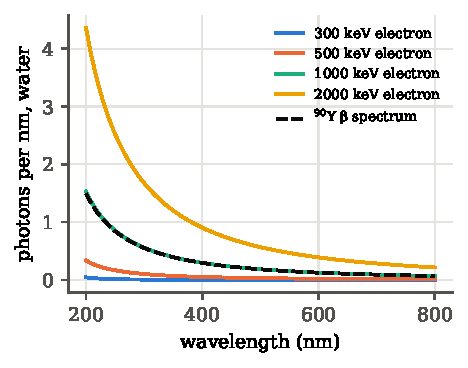
\includegraphics[width=0.62\linewidth]{fig/c_spec.pdf}
\caption{Cherenkov photons per nm in water for mono-energetic electrons and for the \nuc{90}{Y} beta spectrum (per decay, dashed). The $1/\lambda^2$ shape is modified by the threshold, which removes photons first at long wavelengths where $n$ is smallest.}
\label{fig:spec}
\end{figure}

\begin{figure}[htbp]
\centering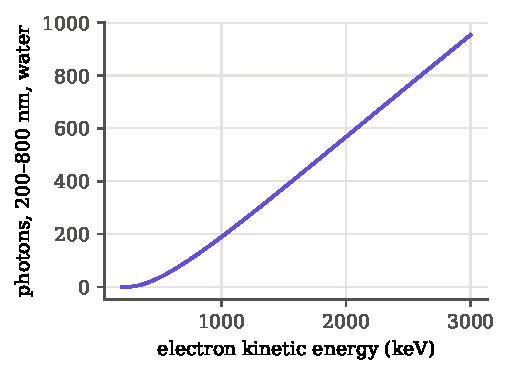
\includegraphics[width=0.55\linewidth]{fig/c_tot.pdf}
\caption{Total photons between 200 and \SI{800}{nm} in water versus electron kinetic energy: zero below \SI{\approx 250}{keV}, about 35 at \SI{500}{keV}, 190 at \SI{1}{MeV} and 840 at \SI{2.7}{MeV}. Well above threshold the yield grows roughly linearly with the energy above threshold, at $\approx 380$ photons per MeV.}
\label{fig:tot}
\end{figure}

\begin{keyidea}[Why Cherenkov light matters for scintillator detectors]
In a liquid-scintillator or liquid-argon detector, Cherenkov light in the PMT glass, acrylic vessel or light guides from \nuc{40}{K}, \nuc{208}{Tl} or \nuc{214}{Bi} decays gives prompt, low-photon-count pulses with almost no late light. They can look like fast scintillation (nuclear-recoil-like in argon pulse-shape discrimination). Estimating them requires exactly \cref{eq:fold}, with the beta and gamma-electron spectra of each contaminant and the transmission of each material.
\end{keyidea}

\section{What the Cherenkov tab outputs}
The photon spectrum per nm (per electron or per decay), the total in the chosen wavelength window, the electron threshold at the centre of the wavelength window, the plot of $n(\lambda)$, the formula, and a CSV with wavelength, $n$, and photons per nm.

\section{Exercises}
\begin{exercise}[A]
Derive \cref{eq:angle} with Huygens' construction, and \cref{eq:thr}. Show that the threshold for muons in water is \SI{55}{MeV} and for protons \SI{0.48}{GeV}.
\end{exercise}
\begin{exercise}[A]
Integrate \cref{eq:ft} for $\beta = 1$ over 300--\SI{600}{nm} with constant $n = 1.33$ and verify the \SI{\approx 330}{photons/cm} quoted above. How much does using the Sellmeier $n(\lambda)$ for water change this?
\end{exercise}
\begin{exercise}[A]
Show that well above threshold $\dd N/\dd\lambda(T_0)$ grows linearly with $T_0$ when $S$ is constant, and estimate the slope in photons per MeV for water using $S\approx\SI{1.85}{MeV\,cm^2/g}$. Compare with \cref{fig:tot}.
\end{exercise}
\begin{exercise}[P]
Reproduce \cref{fig:tot} with your own implementation of \cref{eq:track}, then add the density-effect correction (Sternheimer parameters for water) and estimate its effect at \SI{3}{MeV}.
\end{exercise}
\begin{exercise}[P]
Using the Beta and Gamma tabs (or their generated code), compute the Cherenkov photons per decay between 300 and \SI{500}{nm} produced in a \SI{5}{mm} borosilicate PMT window by \nuc{40}{K} (both the $\beta^-$ branch and the \SI{1461}{keV} gamma). Which contribution dominates, and what assumption in the gamma part is most questionable for a thin window?
\end{exercise}
\begin{exercise}[R]
Design a measurement that separates Cherenkov from scintillation light in a water-based liquid scintillator using timing, direction and spectrum. Which of these does \cref{eq:ft} predict, and which require the detector simulation?
\end{exercise}

\begin{thebibliography}{9}
\bibitem{jelley} J.~V. Jelley, \emph{\v{C}erenkov Radiation and its Applications} (Pergamon, 1958).
\bibitem{jackson} J.~D. Jackson, \emph{Classical Electrodynamics}, 3rd ed.\ (Wiley, 1999), sec.~13.4.
\bibitem{icru37} ICRU Report 37, \emph{Stopping Powers for Electrons and Positrons} (1984).
\bibitem{daimon} M.~Daimon and A.~Masumura, ``Measurement of the refractive index of distilled water from the near-infrared region to the ultraviolet region'', Appl.\ Opt.\ \textbf{46}, 3811 (2007).
\bibitem{malitson} I.~H. Malitson, ``Interspecimen comparison of the refractive index of fused silica'', J.\ Opt.\ Soc.\ Am.\ \textbf{55}, 1205 (1965).
\bibitem{pdg} Particle Data Group, ``Passage of particles through matter'', in R.~L. Workman \emph{et al.}, Prog.\ Theor.\ Exp.\ Phys.\ \textbf{2022}, 083C01, and later editions.
\end{thebibliography}
\end{document}
